\documentclass{article}

\usepackage[colorlinks, urlcolor=blue, linkcolor=red, citecolor=green]{hyperref}
\usepackage{fancyhdr} %设置页眉和页脚的
\usepackage{extramarks} %设置continue那玩意的
\usepackage{amsmath}
\usepackage{amsthm}
\usepackage{amsfonts}
\usepackage{tikz} %画线的
\usepackage[plain]{algorithm}
\usepackage{algpseudocode}
\usepackage{enumerate}

\usetikzlibrary{automata,positioning}

%表
\usepackage{booktabs}
\usepackage{multirow}
\usepackage{array}
\usepackage{caption}
\DeclareCaptionFont{heiti}{\heiti} %还可以定义其他的
\captionsetup{labelsep=space, font={small, bf}, skip=2pt} %space可以改成quad

%图
%*****************图片及其相关设置***************************
\usepackage{graphicx}
\graphicspath{{tupian/}}
\usepackage{subfigure}
%

%*****************代码相关设置***************************
\usepackage{pythonhighlight}

\usepackage{dsfont}
% Basic Document Settings
%

\topmargin=-0.45in
\evensidemargin=0in
\oddsidemargin=0in
\textwidth=6.5in
\textheight=9.0in
\headsep=0.25in

\linespread{1.1}

\pagestyle{fancy}
\lhead{\hmwkAuthorName}
\chead{\hmwkClass: \hmwkTitle}
\rhead{\firstxmark}
\lfoot{\lastxmark}
\cfoot{\thepage}

\renewcommand\headrulewidth{0.4pt}
\renewcommand\footrulewidth{0.4pt}

\setlength\parindent{0pt}

%
% Create Problem Sections
%

\newcommand{\enterProblemHeader}[1]{
    \nobreak\extramarks{}{Assignment A3.\arabic{#1} continued on next page\ldots}\nobreak{}
    \nobreak\extramarks{Assignment A3.\arabic{#1} (continued)}{Assignment A3.\arabic{#1} continued on next page\ldots}\nobreak{}
}

\newcommand{\exitProblemHeader}[1]{
    \nobreak\extramarks{Assignment A3.\arabic{#1} (continued)}{Assignment A3.\arabic{#1} continued on next page\ldots}\nobreak{}
    \stepcounter{#1}
    \nobreak\extramarks{Assignment A3.\arabic{#1}}{}\nobreak{}
}

\setcounter{secnumdepth}{0}
\newcounter{partCounter}
\newcounter{homeworkProblemCounter}
\setcounter{homeworkProblemCounter}{1}
\nobreak\extramarks{Assignment A3.\arabic{homeworkProblemCounter}}{}\nobreak{}

\newenvironment{homeworkProblem}{
    \section{Assignment A3.\arabic{homeworkProblemCounter}}
    \setcounter{partCounter}{1}
    \enterProblemHeader{homeworkProblemCounter}
}{
    \exitProblemHeader{homeworkProblemCounter}
}

%
% Homework Details
%   - Title
%   - Due date
%   - Class
%   - Section/Time
%   - Instructor
%   - Author
%

\newcommand{\hmwkTitle}{Homework\ \#3}
\newcommand{\hmwkDueDate}{November 20, 2020}
\newcommand{\hmwkClass}{Introduction to Optimization}
\newcommand{\hmwkClassTime}{}
\newcommand{\hmwkClassInstructor}{Professor Andre Milzarek}
\newcommand{\hmwkAuthorName}{Peng Deng}
\newcommand{\hmwkAuthorSchool}{School of Data Science}
\newcommand{\hmwkAuthorNumber}{Sno.220041042}
%
% Title Page
%

\title{
    \vspace{2in}
    \textmd{\textbf{\hmwkClass:\ \hmwkTitle}}\\
    \normalsize\vspace{0.1in}\small{Due\ on\ \hmwkDueDate}\\
    \vspace{0.1in}\large{\textit{\hmwkClassInstructor\ \hmwkClassTime}}
    \vspace{3in}
}

\author{\textbf{\hmwkAuthorName}}

\date{}

\renewcommand{\part}[1]{\textbf{\large Part \Alph{partCounter}}\stepcounter{partCounter}\\}

%
% Various Helper Commands
%

% Useful for algorithms
\newcommand{\alg}[1]{\textsc{\bfseries \footnotesize #1}}

% For derivatives
\newcommand{\deriv}[1]{\frac{\mathrm{d}}{\mathrm{d}x} (#1)}

% For partial derivatives
\newcommand{\pderiv}[2]{\frac{\partial}{\partial #1} (#2)}

% Integral dx
\newcommand{\dx}{\mathrm{d}x}

% Alias for the Solution section header
\newcommand{\solution}{\textbf{\large Solution}}

% Probability commands: Expectation, Variance, Covariance, Bias
\newcommand{\E}{\mathrm{E}}
\newcommand{\Var}{\mathrm{Var}}
\newcommand{\Cov}{\mathrm{Cov}}
\newcommand{\Bias}{\mathrm{Bias}}
\begin{document}

\maketitle
\thispagestyle{empty}

\newpage
\setcounter{page}{1}

\begin{homeworkProblem}
In this first exercise, we investigate the performance of the bisection and golden section method.
\begin{enumerate}[a)]
	\item We consider the optimization problem
	\begin{equation}
		\min_x f(x):=\frac{x^2}{10}-2\sin(x)\quad \text { s.t. }\quad x\in[0,4].
	\end{equation}
	Implement the golden section method to solve this problem and output a solution with accuracy at least $10^{-5}$.
	\item Consider the minimization problem
	$$
	\min _{x \in \mathbb{R}} g(x) \quad \text { s.t. } \quad x \in[0,1],
	$$
	where $g$ is given by $g(x):=e^{-x}-\cos (x) .$ Solve this problem using the bisection and the golden section method. Compare the number of iterations required to recover a solution in [0,1] with accuracy less or equal than $10^{-5}$
\end{enumerate}

\vspace{4pt}
\textbf{\large{Solution}}

\vspace{4pt}
\textbf{Subproblem (a)}

By implementing the golden section method, we can obtain the solution as $x=1.42755$ after 27 iterations. The python code to solve this problem is showing in as follow.
\begin{python}
	import numpy as np
	# f(x) = x^2/10 - 2*sin(x)
	def f(x):
		return x**2/10 - 2*np.sin(x)
	xl = 0
	xr = 4
	fi = (3 - np.sqrt(5)) / 2
	gap = 1e-5
	num_iteration = 0
	last_update = 0 #0:left; 1:right
	while (xr - xl) >= gap:
		if num_iteration == 0:
			new_xl = fi * xr + (1 - fi) * xl
			new_xr = (1 - fi) * xr + fi * xl
		elif last_update == 0:
			new_xl = new_xr
			new_xr = (1 - fi) * xr + fi * xl
		else:
			new_xr = new_xl
			new_xl = fi * xr + (1 - fi) * xl
		
		f_xl = f(new_xl)
		f_xr = f(new_xr)
		
		if f_xl < f_xr:
			xr = new_xr
			last_update = 1
		else:
			xl = new_xl
			last_update = 0
		num_iteration = num_iteration + 1
		
	ans = (xl + xr) / 2
	print('x=', ans)
	print('number of iterations:', num_iteration)
\end{python}
\vspace{4pt}
\textbf{Subproblem (b)}

$\circ$ By implementing the golden section method, we can obtain the solution as $x=0.58853$ after 24 iterations. By implementing the bisection method, we can obtain the solution as $x=0.58853$ after 17 iterations. The python code to solve this problem is showing as follow.
\begin{python}
	import numpy as np
	def f(x):
		return np.e**(-x) - np.cos(x)
	def df(x):
		return -np.e**(-x) + np.sin(x)
	xl = 0
	xr = 1
	gap = 1e-5
	
	#golden section
	fi = (3 - np.sqrt(5)) / 2
	num_iteration = 0
	last_update = 0 #0:left; 1:right
	while (xr - xl) >= gap:
		if num_iteration == 0:
			new_xl = fi * xr + (1 - fi) * xl
			new_xr = (1 - fi) * xr + fi * xl
		elif last_update == 0:
			new_xl = new_xr
			new_xr = (1 - fi) * xr + fi * xl
		else:
			new_xr = new_xl
			new_xl = fi * xr + (1 - fi) * xl
		
		f_xl = f(new_xl)
		f_xr = f(new_xr)
		
		if f_xl < f_xr:
			xr = new_xr
			last_update = 1
		else:
			xl = new_xl
			last_update = 0
		num_iteration = num_iteration + 1
	
	ans = (xl + xr) / 2
	print('------golden section---------')
	print('x=', ans)
	print('number of iterations:', num_iteration)
	
	# bisection
	num_iteration = 0
	xl = 0
	xr = 1
	while (xr - xl) >= gap:
		xm = (xl + xr) / 2
		if df(xm) == 0:
			break
		if df(xm) > 0:
			xr = xm
		else:
			xl = xm
		num_iteration = num_iteration + 1
	print('------bisection---------')
	print('x=', ans)
	print('number of iterations:', num_iteration)
\end{python}



\end{homeworkProblem}

\begin{homeworkProblem}
	Let $f: \mathbb{R}^{n} \rightarrow \mathbb{R}$ be a continuously differentiable function and consider $x \in \mathbb{R}^{n}$ with $\nabla f(x) \neq 0$. Verify the following statements:
	\begin{itemize}
		\item[a)] Set $d=-\left(\nabla f(x)_{j}\right) \cdot e_{j}=-\frac{\partial f}{\partial x_{j}}(x) \cdot e_{j},$ where $e_{j} \in \mathbb{R}^{n}$ is the $j$ -th unit vector and $j \in\{1, \ldots, n\}$
		is an index satisfying
		$$
		\left|\frac{\partial f}{\partial x_{j}}(x)\right|=\max _{1 \leq i \leq n}\left|\frac{\partial f}{\partial x_{i}}(x)\right|=\|\nabla f(x)\|_{\infty}
		$$
		Then $d$ is a descent direction of $f$ at $x$.
		\item[b)] Let us define $d=-\nabla f(x) / \sqrt{\varepsilon+\|\nabla f(x)\|^{2}}$. Show that $d$ is a descent direction of $f$ at $x$.
		\item[c)] Suppose that $f$ is twice continuously differentiable and define $d_{i}=-\left(\nabla f(x)_{i}\right) /\left(\nabla^{2} f(x)_{i i}\right)$ for all $i \in\{1, \ldots, n\} .$ If $\nabla^{2} f(x)$ is positive definite, then $d$ is well-defined (we do not divide by zero) and it is a descent direction of $f$ at $x$.
	\end{itemize}
\end{homeworkProblem}

\vspace{4pt}
\textbf{\large{Solution}}

\vspace{4pt}
\textbf{Subproblem (a)}

In order to verify $d$ is a descent direction of $f$ at $x$, we have to verify $\nabla f(x)^{\top}d<0$.
\begin{equation}
	\begin{split}
		\nabla f(x)^{\top}d&=-\nabla f(x)^{\top}\frac{\partial f}{\partial x_{j}}(x) \cdot e_{j}\\
		&=-
		\begin{pmatrix}
			\frac{\partial f}{\partial x_{1}}&\frac{\partial f}{\partial x_{2}} \cdots \frac{\partial f}{\partial x_{n}}
		\end{pmatrix}
		\begin{pmatrix}
			0\\
			\vdots\\
			\frac{\partial f}{\partial x_{j}}\\
			\vdots\\
			0
		\end{pmatrix}\\
		&=-\left(\frac{\partial f}{\partial x_{j}}\right)^2
	\end{split}
\end{equation}
Because we know $\nabla f(x) \neq 0$, and $j \in\{1, \ldots, n\}$
is an index satisfying
	$$
		\left|\frac{\partial f}{\partial x_{j}}(x)\right|=\max _{1 \leq i \leq n}\left|\frac{\partial f}{\partial x_{i}}(x)\right|=\|\nabla f(x)\|_{\infty}
	$$
So we can conclude that $\frac{\partial f}{\partial x_{j}}\neq 0$, because if $\frac{\partial f}{\partial x_{j}}=0$, then for $\forall i, \frac{\partial f}{\partial x_{i}}= 0$, so the gradient will be 0, which is an contradiction. Thus, $\frac{\partial f}{\partial x_{j}}\neq 0$, and $-\left(\frac{\partial f}{\partial x_{j}}\right)^2 <0$. Then, $\nabla f(x)^{\top}d<0$, which means $d$ is a descent direction of $f$ at $x$.

\vspace{4pt}
\textbf{Subproblem (b)}

We can derive 
\begin{equation}
	\begin{split}
		\nabla f(x)^{\top}d&=-\frac{1}{\sqrt{\varepsilon+\|\nabla f(x)\|^{2}}}f(x)^{\top}\nabla f(x)\\
		&=-\frac{1}{\sqrt{\varepsilon+\|\nabla f(x)\|^{2}}}\|\nabla f(x)\|^{2}<0
	\end{split}
\end{equation}
Thus, we verified that $d$ is a descent direction of $f$ at $x$.
\pagebreak

\vspace{4pt}
\textbf{Subproblem (c)}

$\circ$ Because we know $\nabla^{2} f(x)$ is positive definite, so we have
\begin{equation}
	\begin{split}
		h^{\top}\nabla^{2} f(x)h>0, \quad\forall h\in\mathbb{R}^n
	\end{split}
\end{equation}
We set $e_{i} \in \mathbb{R}^{n}$ is the $i$ -th unit vector and $i \in\{1, \ldots, n\}$. So we have 
\begin{equation}
	\begin{split}
		e_i^{\top}\nabla^{2}f(x)e_i=\nabla^{2} f(x)_{i i}>0
	\end{split}
\end{equation}
Thus, we do not divided by zero because $\nabla^{2} f(x)_{i i}>0$.

$\circ$ For the direction $d$, we can derive
\begin{equation}
	\begin{split}
		\nabla f(x)^{\top}d&=-
		\begin{pmatrix}
			\frac{\partial f}{\partial x_{1}}&\frac{\partial f}{\partial x_{2}} \cdots \frac{\partial f}{\partial x_{n}}
		\end{pmatrix}
		\begin{pmatrix}
			\nabla f(x)_{1}/\nabla^{2} f(x)_{1 1}\\
			\vdots\\
			\nabla f(x)_{i}/\nabla^{2} f(x)_{i i}\\
			\vdots\\
			\nabla f(x)_{n}/\nabla^{2} f(x)_{n n}
		\end{pmatrix}\\
		&=-\sum_{i=1}^{n}\frac{\left(\nabla f(x)_{i}\right)^2}{\nabla^{2} f(x)_{i i}}<0 \qquad \left(\text{Because: } \nabla f(x)\neq 0\right)
	\end{split}
\end{equation}
Thus, we have verified that $d$ is a descent direction of $f$ at $x$.
\begin{homeworkProblem}
	Implement the gradient descent method (Lecture L-06, slide 23) that was presented in the lecture as a function gradient\_method in \textbf{MATLAB} or \textbf{Python}.
	
	\vspace{4pt}
	
	The following input functions and parameters should be considered:
	
	\begin{itemize}
		\item obj, grad - function handles that calculate and return the objective function $f(x)$ and the gradient $\nabla f(x)$ at an input vector $x \in \mathbb{R}^{n}$. You can treat these handles as functions or fields of a class or structure $\mathrm{f}$ or use them directly as input. (For example, your function can have the form gradient\_method (obj, grad,....)).
		
		\item $x^{0}-$ the initial point.
		
		\item tol - a tolerance parameter. The method should stop whenever the current iterate $x^{k}$ satisfies the criterion $\left\|\nabla f\left(x^{k}\right)\right\| \leq$ tol.
		
	\end{itemize}
	
	We want to analyze the performance of the gradient method for different step size strategies. In particular, we want to test and compare backtracking, exact line search, and diminishing step sizes. The following parameters will be relevant for these strategies:
	\begin{itemize}
		\item $s>0, \sigma, \gamma \in(0,1)-$ parameters for backtracking and the Armijo condition.
		\item alpha - a function that returns a pre-defined, diminishing step size $\alpha_{k}=$ alpha (k) satisfying $\alpha_{k} \rightarrow 0$ and $\sum \alpha_{k}=\infty$
		\item You can use the golden section method from Assignment A3.1 to determine the exact step size $\alpha_{k} .$ The parameters for the golden section method are: maxit (maximum number of iterations), tol (stopping tolerance), $[0, \mathrm{a}]$ (the interval of the step size).
	\end{itemize}
	
	You can organize the latter parameters in an appropriate options class or structure. It is also possible to implement two separate algorithms for backtracking and diminishing step sizes. The method(s) should return the final iterate $x^{k}$ that satisfies the stopping criterion.
	
	\begin{itemize}
		\item[a)] Test your implementation on the following problem:
		$$
		\min _{x \in \mathbb{R}^{2}} f(x)=f_{1}(x)^{2}+f_{2}(x)^{2}
		$$
		where $f_{1}: \mathbb{R}^{2} \rightarrow \mathbb{R}$ and $f_{2}: \mathbb{R}^{2} \rightarrow \mathbb{R}$ are given by:
		$$
		\begin{array}{l}
		f_{1}(x):=3+x_{1}+\left(\left(1-x_{2}\right) x_{2}-2\right) x_{2} \\
		f_{2}(x):=3+x_{1}+\left(x_{2}-3\right) x_{2}
		\end{array}
		$$
		- Calculate all stationary points of the function $f$ and analyze which of the points are (global/local) minimizer, (global/local) maximizer, or saddle points.
		
		\textbf{Hint}: This problem has five stationary points.
		
		- Apply the gradient method with backtracking and parameters $(s, \sigma, \gamma)=(1,0.5,0.1)$ with diminishing step sizes
		$$
		\alpha_{k}=\frac{0.01}{\log (k+2)}
		$$
		and exact line search (maxit $=100,$ tol $=10^{-6}, \mathrm{a}=2$ ) to solve the problem $\min _{x} f(x)$.
		
		The algorithms should use the stopping tolerance tol $=10^{-5}$. Test the methods using the initial point $(0,0)^{\top}$ and report the behavior and performance of the methods. In particular, for each of the initial points, compare the number of iterations and the point to which each algorithm converged.
	\end{itemize}
	\begin{itemize}
		\item[b)] Adjust your code such that the norm of the gradients, $\left\|\nabla f\left(x^{k}\right)\right\|,$ are saved and returned. Plot the sequences $\left(\left\|\nabla f\left(x^{k}\right)\right\|\right)_{k}$ and $\left(\left\|x^{k}-x^{*}\right\|\right)_{k}$ (with the iteration number $k$ as $x$ -axis) in a logarithmic scale and compare the performance of the gradient method using the different step size strategies mentioned in part a). Here, $x^{*}$ denotes the limit point of the sequence generated by the gradient method. Which type of convergences can be observed?
		
		\item[c)] Let us define the set(this is a rectangle).
		$$
		\mathcal{X}^{0}:=\left\{x \in \mathbb{R}^{2}: x_{1} \in\{-10,10\}, x_{2} \in[-2,2]\right\} \cup\left\{x \in \mathbb{R}^{2}: x_{1} \in\right.
		\left.[-10,10], x_{2} \in\{-2,2\}\right\}
		$$
		Run the methods:
		\begin{itemize}
			\item[-] Gradient descent method with backtracking and $(s, \sigma, \gamma)=(1,0.5,0.1)$
			\item[-] Gradient method with diminishing step sizes $\alpha_{k}=0.01 / \log (k+2)$
			\item[-] Gradient method with exact line search and maxit $=100,$ tol $=10^{-6}, \mathrm{a}=2$
		\end{itemize}
		again with $p$ different initial points selected from the set $\mathcal{X}^{0}$. The initial points should uniformly cover the different parts of the set $\mathcal{X}^{0}$ and you can use the tolerance tol $=10^{-5}$ and $p \in[10,20] \cap \mathbb{N} .$ For each algorithm create a single figure that contains all of the solution paths generated for the different initial points. The initial points and limit points should be clearly visible. Add a contour plot of the function $f$ in the background of each figure.
		
		\textbf{Hint}: You might need to adjust the diminishing step sizes to still guarantee convergence.
	\end{itemize}

\vspace{4pt}
\textbf{\large{Solution}}

\vspace{4pt}
\textbf{Subproblem (a)}

$\circ$ Part 1: The calculation of stationary points.

The gradient of function $f$ is as follow:
\begingroup
\renewcommand*{\arraystretch}{1.5}
\begin{equation}
	\begin{split}
		\nabla f(x)&=
		\begin{pmatrix}
			\frac{\partial f}{\partial x_1}\\
			\vspace{2pt}
			\frac{\partial f}{\partial x_2}
		\end{pmatrix}
		=
		\begin{pmatrix}
			2f_1(x)+2f_2(x)\\
			2f_1(x)(2x_2-3x_2^2-2)+2f_2(x)(2x_2-3)
		\end{pmatrix}
		\\
	\end{split}
\end{equation}
\endgroup
The Hessian of function $f$ is as follow:
\begingroup
\renewcommand*{\arraystretch}{1.5} 
\begin{equation}
	\begin{split}
		\nabla^2 f(x)&=
		\begin{pmatrix}
			\frac{\partial^2 f}{\partial x_1\partial x_1}&
			\frac{\partial^2 f}{\partial x_1\partial x_2}\\
			\frac{\partial^2 f}{\partial x_2\partial x_1}&
			\frac{\partial^2 f}{\partial x_2\partial x_2}
		\end{pmatrix}
		=
		\begin{pmatrix}
			4&8x_2-6x_2^2-10\\
			8x_2-6x_2^2-10&2f_1(x)(-6x_2+2)+2(2x_2-3x_2^2-2)^2+4f_2(x)+2(2x_2-3)^2
		\end{pmatrix}
		\\
	\end{split}
\end{equation}
\endgroup
By solving the equation $\nabla f(x)=0$, we derive the stationary points as follow:
$$
A(-7,-1)\quad B(-3,0)\quad C(-1,1)\quad D\left(-\frac{2}{9}\left(15+4\sqrt{3}\right), -\frac{1}{\sqrt{3}}\right)\quad E\left(\frac{2}{9}\left(4\sqrt{3}-15\right), \frac{1}{\sqrt{3}}\right)
$$
By calculating the Hessian matrix for point $ A, B, C, D, E $, we can find that at points $A, B, C$, the Hessian matrix is positive definite, and at points $D, E$, the Hessian matrix is indefinite. Thus, points $A, B, C$ are strict local minimizer, and points $D, E$ are saddle points.

We can calculate the value as $f(A)=f(B)=f(C)=0$. Because $f(x)=f_{1}(x)^{2}+f_{2}(x)^{2}$, so $f(x)\geq 0$, and it is continuous and differentiable. So points $A,B,C$ are all global minimizer, but not strict.

Thus, points $A,B,C$ are strict local minimizer and global minimizer (not strict). Points $D, E$ are saddle points.

$\circ$ Part 2: The gradient method

By using different step size strategies (Backtracking, Exact line search and Diminishing step size method), we find that with the initial point (0, 0), all the method converges to the point (-1, 1) approximately. The number of iterations with different step size strategies are 162 (Backtracking), 11993 (Diminishing step size), and 7 (Exact line search). As we can see from the result, "Exact line search" is the fastest method, and "Diminishing step size" is the lowest method for this certain problem. The python code to solve this problem is as follow:
\begin{python}
import numpy as np

def f1(x):
	return 3 + x[0] + ((1 - x[1]) * x[1] - 2) * x[1]
def f2(x):
	return 3 + x[0] + (x[1] - 3) * x[1]
def f(x):
	return f1(x) * f1(x) + f2(x) *f2(x)
def df(x):
	grad = np.zeros(2).reshape(2,1)
	grad[0] = 2 * f1(x) + 2 * f2(x)
	grad[1] = 2 * f1(x) * (2*x[1] - 3*(x[1]**2) - 2) + 2 * f2(x) * (2*x[1] - 3)
	return grad
def norm(x):
	return np.sqrt(x[0]**2 + x[1]**2)

#backtracking method
s = 1
sigma = 0.5
gamma = 0.1
alpha = s
tol = 1e-5

initial = np.array([0, 0]).reshape(2, 1)
xk = initial
gradient = df(xk)
num_iteration = 0

while norm(gradient) > tol:
	alphak = s
	dk = -df(xk)
	while True:
		if f(xk + alphak*dk) - f(xk) <= gamma * alphak * np.dot(df(xk).T, dk):
			break
		alphak = alphak * sigma
	xk = xk + alphak * dk
	gradient = df(xk)
	num_iteration = num_iteration + 1
print('--------backtracking---------')
print('xk:\n', xk)
print('number of iterations:', num_iteration)
print()

#diminishing step size
def alpha_k(k):
	return 0.01/(np.log(k+2))

num_iteration = 0
k = 1
xk = initial
gradient = df(xk)

while norm(gradient) > tol:
	dk = -df(xk)
	alphak = alpha_k(k)
	xk = xk + alphak * dk
	gradient = df(xk)
	num_iteration = num_iteration + 1
	k = k + 1
print('--------diminishing step size---------')
print('xk:\n', xk)
print('number of iterations:', num_iteration)
print()

# exact line search
tol_golden = 1e-6
maxit = 100
a = 2
num_iteration = 0
xk = initial
gradient = df(xk)

while norm(gradient) > tol:
	dk = -df(xk)
	alphal = 0
	alphar = a
	num_iteration_golden = 0
	last_update = 0 #0:left; 1:right
	fi = (3 - np.sqrt(5)) / 2
	while (alphar - alphal) >= tol_golden and num_iteration_golden < 100:
		if num_iteration_golden == 0:
			new_alphal = fi * alphar + (1 - fi) * alphal
			new_alphar = (1 - fi) * alphar + fi * alphal
		elif last_update == 0:
			new_alphal = new_alphar
			new_alphar = (1 - fi) * alphar + fi * alphal
		else:
			new_alphar = new_alphal
			new_alphal = fi * alphar + (1 - fi) * alphal
		
		f_alphal = f(xk + new_alphal*dk)
		f_alphar = f(xk + new_alphar*dk)
		
		if f_alphal < f_alphar:
			alphar = new_alphar
			last_update = 1
		else:
			alphal = new_alphal
			last_update = 0
		num_iteration_golden = num_iteration_golden + 1
	alphak = (alphal + alphar) / 2
	xk = xk + alphak * dk
	gradient = df(xk)
	num_iteration = num_iteration + 1
print('--------eaxct line search---------')
print('xk:\n', xk)
print('number of iterations:', num_iteration)
print()  
\end{python}

\vspace{4pt}
\textbf{Subproblem (b)}

From problem (a), we know the limit points of all the three sequences generated by gradient method with different step size method are (-1, 1). So $x^*:=(-1,1)$. The figure of $\left(\left\|\nabla f\left(x^{k}\right)\right\|\right)_{k}$ and $\left(\left\|x^{k}-x^{*}\right\|\right)_{k}$ can be seen in Figure \ref{gradient}.
\begin{figure}[htbp]
	\centering
	\subfigure[$\log\|\nabla f(x^k)\|$ VS number of iteration]{\label{threeD}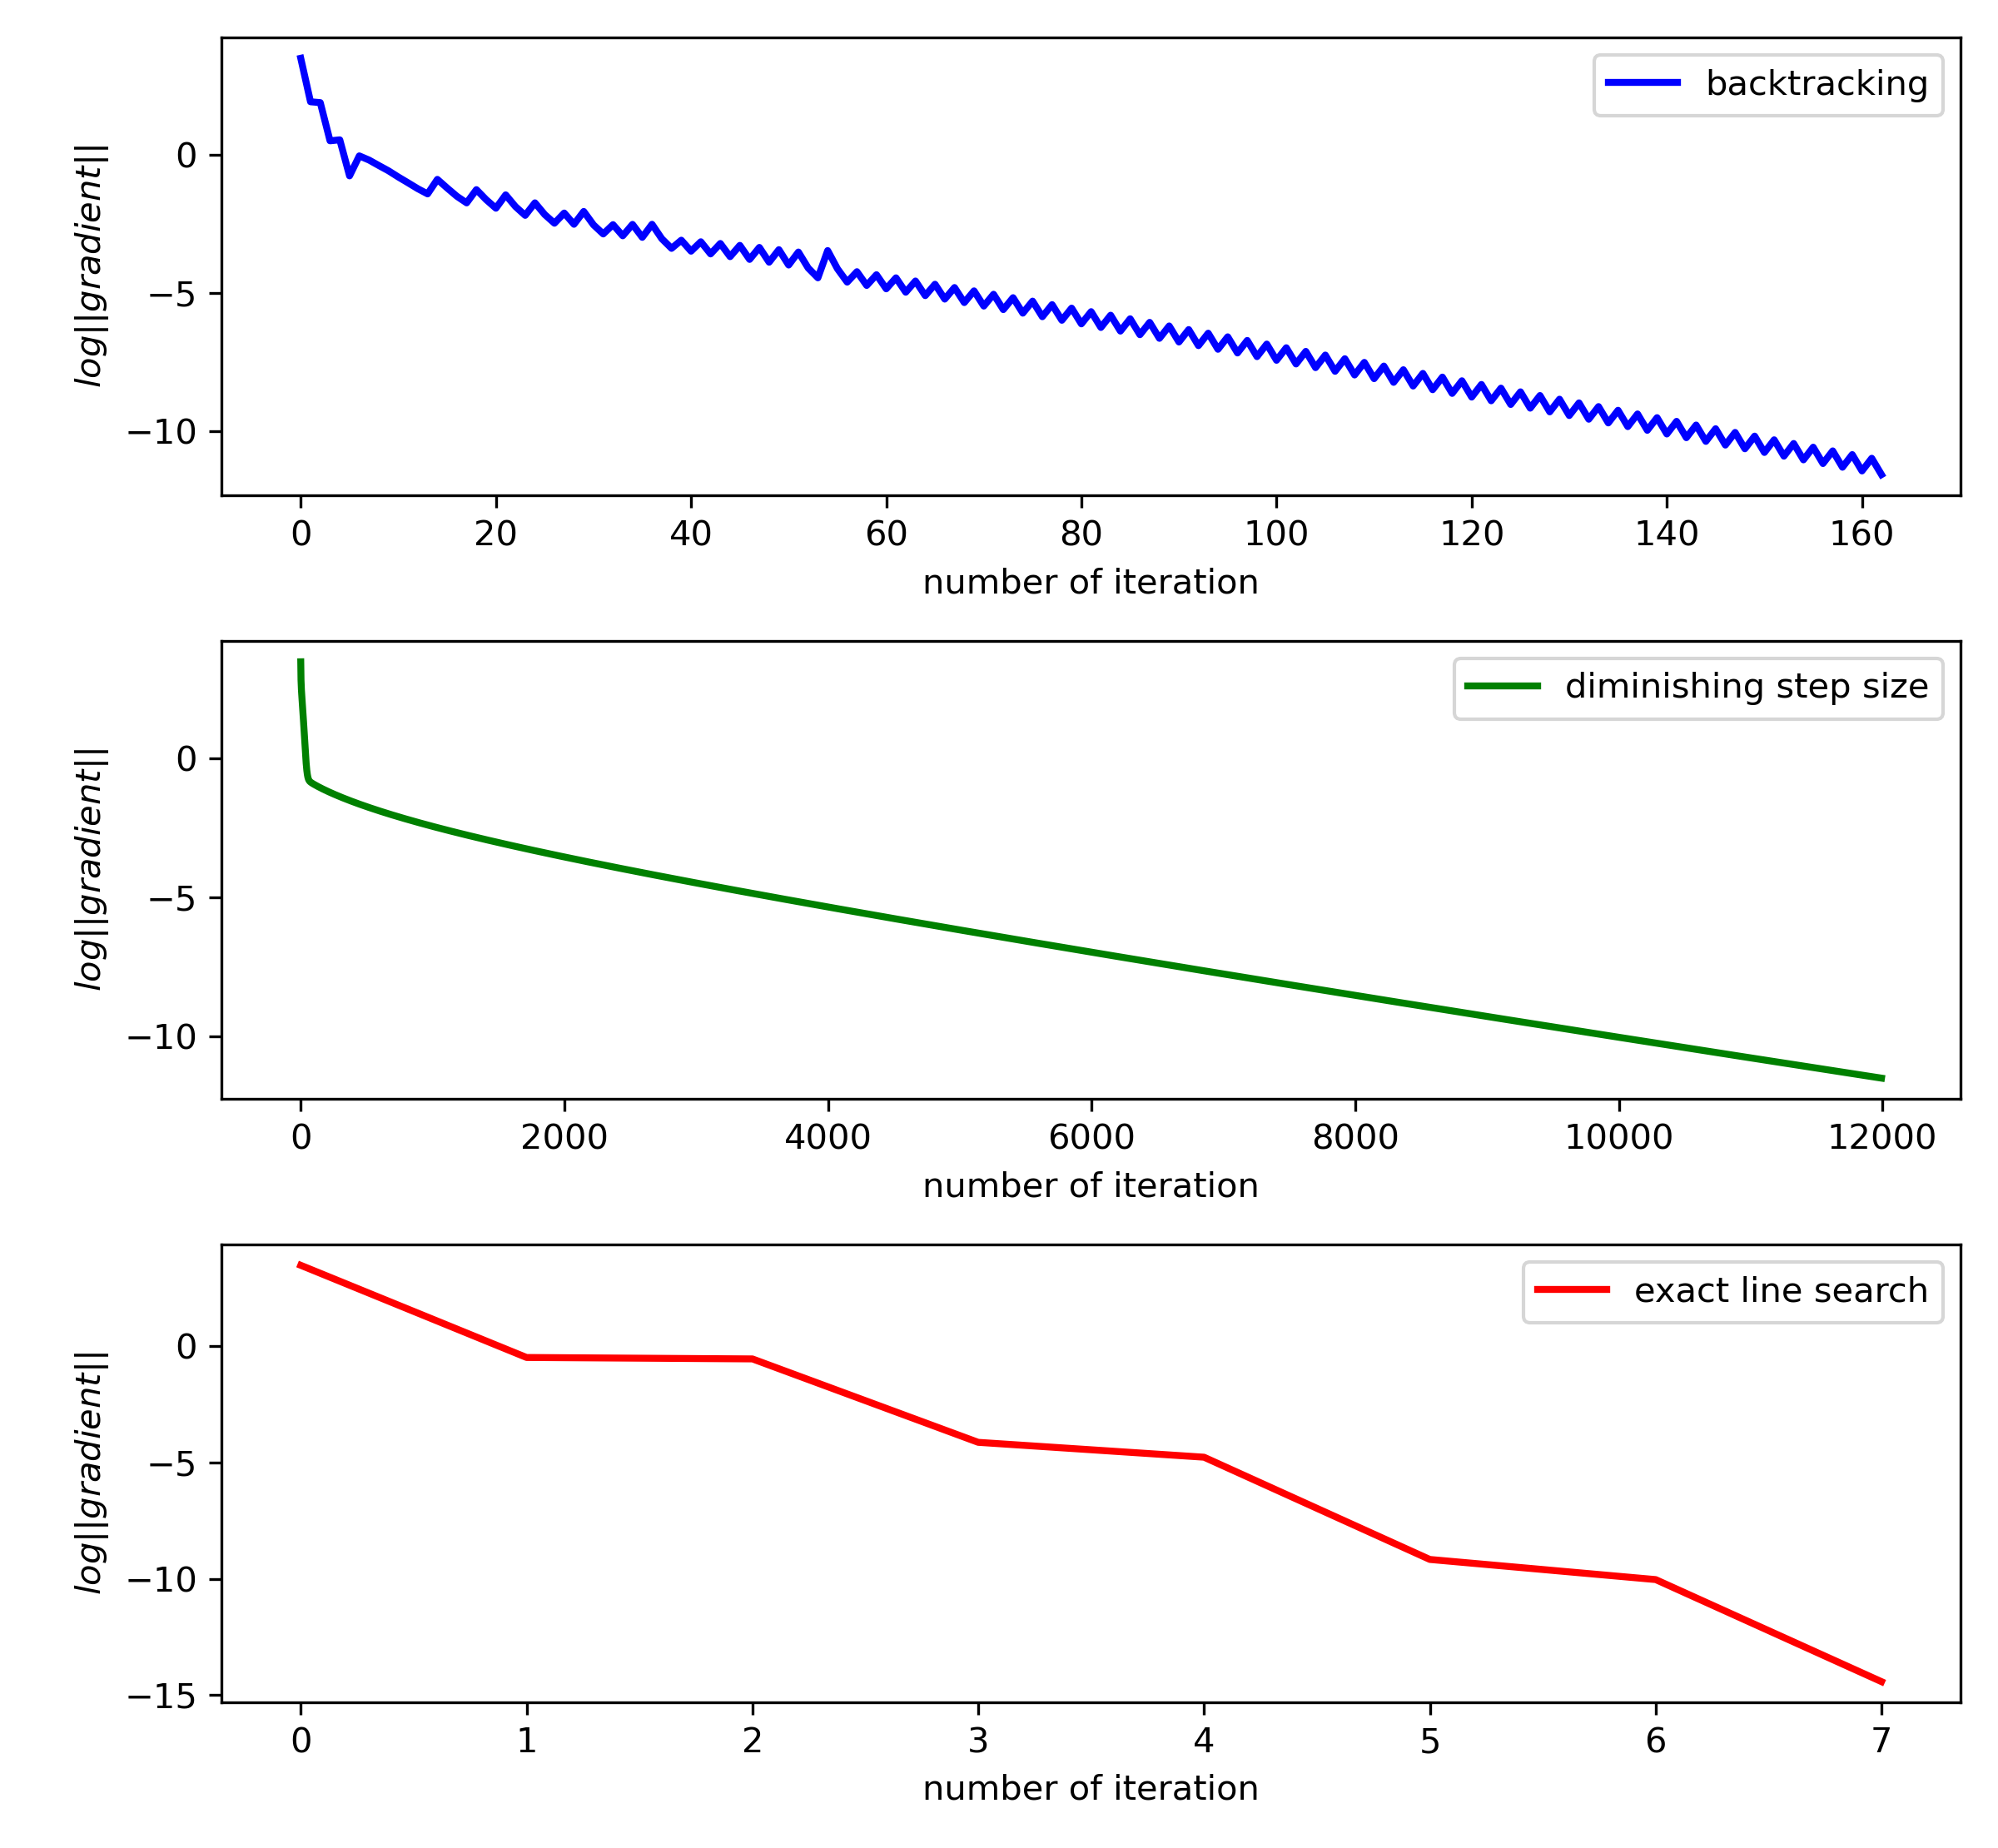
\includegraphics[width=0.47\linewidth]{gradient}}
	\quad
	\subfigure[$\log\|x^k-x^*\|$ VS number of iteration]{\label{contour}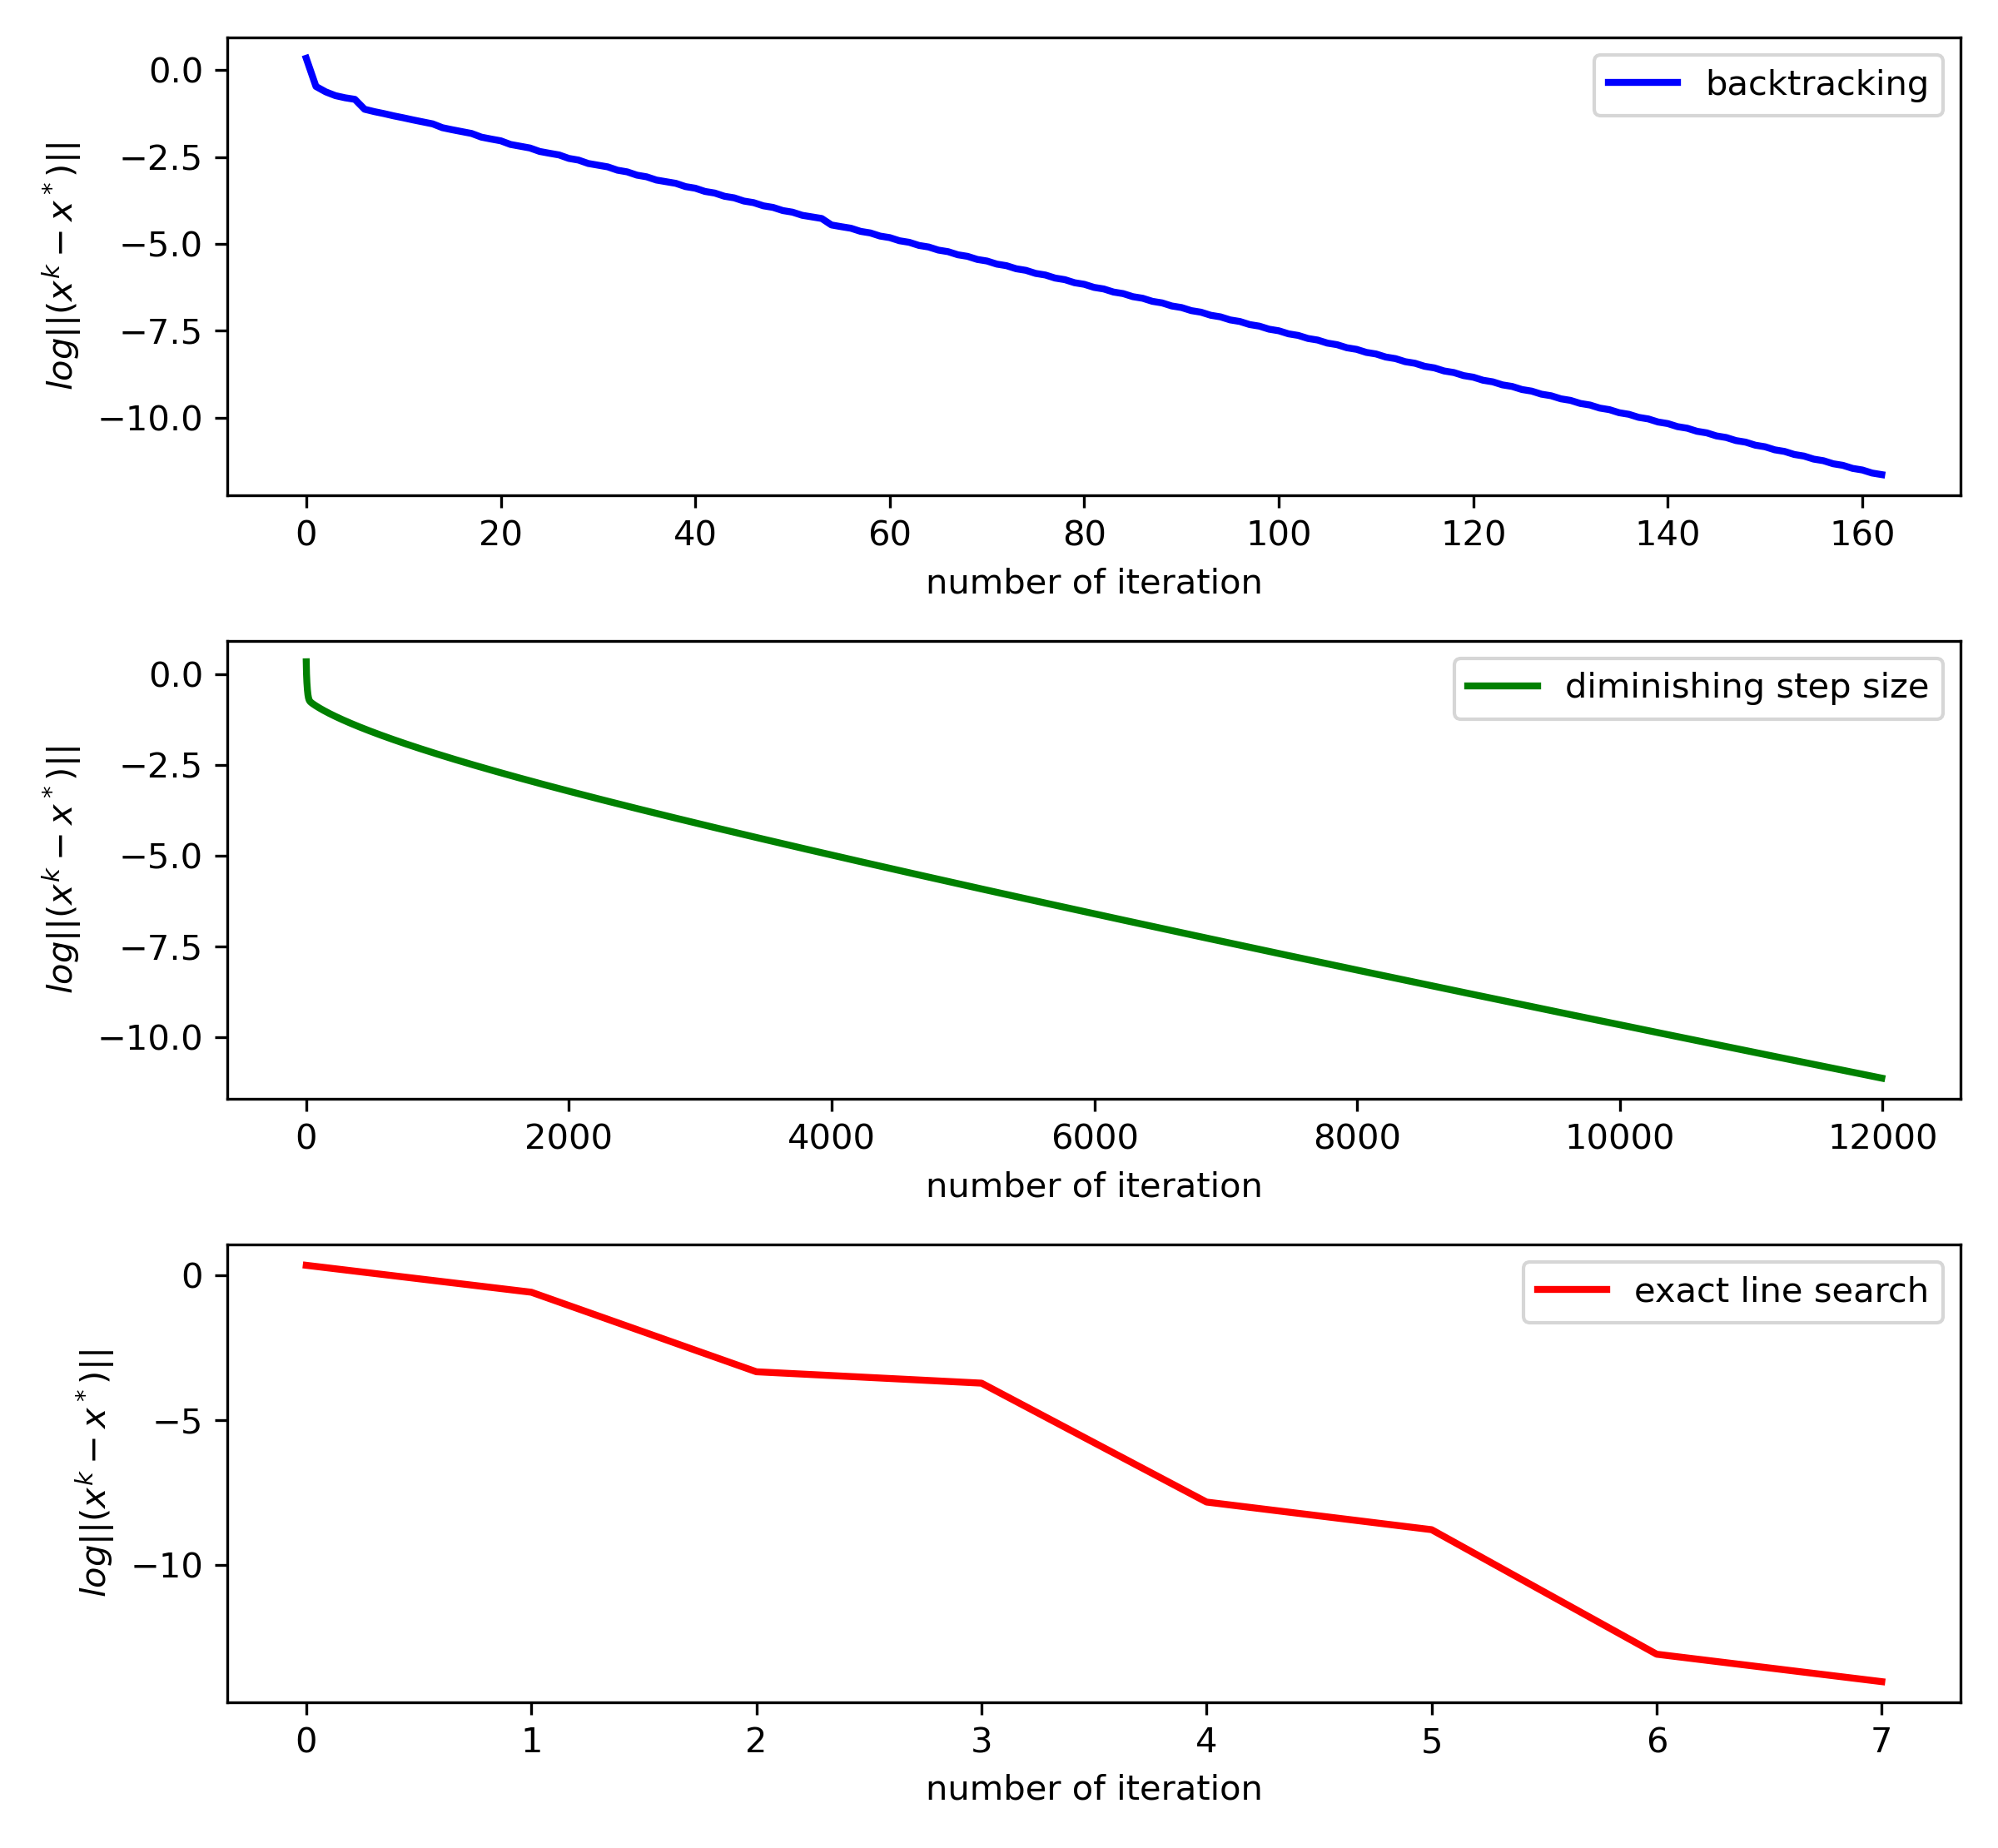
\includegraphics[width=0.47\linewidth]{xk}}
	\caption{The plot of iteration process}
	\label{gradient}
\end{figure}

As we can see from the figure, the convergence type is linear convergence.

The python code to solve this problem is showing below. 
\pagebreak
\begin{python}
import numpy as np
import matplotlib.pyplot as plt

def f1(x):
    return 3 + x[0] + ((1 - x[1]) * x[1] - 2) * x[1]
def f2(x):
    return 3 + x[0] + (x[1] - 3) * x[1]
def f(x):
    return f1(x) * f1(x) + f2(x) *f2(x)
def df(x):
    grad = np.zeros(2).reshape(2,1)
    grad[0] = 2 * f1(x) + 2 * f2(x)
    grad[1] = 2 * f1(x) * (2*x[1] - 3*(x[1]**2) - 2) + 2 * f2(x) * (2*x[1] - 3)
    return grad
def norm(x):
    return np.sqrt(x[0]**2 + x[1]**2)
color_list = ['blue', 'green', 'red', 'cyan']
def plot_gradient(y, method, subfig_num):
    plt.figure(1, figsize=(8,10))
    plt.subplot(3,1,subfig_num)
    n = y.size
    x = np.arange(n)
    y = np.log(y)
    plt.plot(x, y, label=method, color = color_list[subfig_num-1], linewidth=2)
    plt.legend()
    plt.xlabel('number of iteration')
    plt.ylabel('$log||gradient||$')
    plt.tight_layout()
    plt.savefig('gradient', dpi=300)
    
def plot_xk(y, method, subfig_num):
    plt.figure(2, figsize=(8,10))
    plt.subplot(3,1,subfig_num)
    n = y.size
    x = np.arange(n)
    y = np.log(y)
    plt.plot(x, y, label = method, color = color_list[subfig_num-1], linewidth=2)
    plt.legend()
    plt.xlabel('number of iteration')
    plt.ylabel('$log||(x^k-x^*)||$')
    plt.tight_layout()
    plt.savefig('xk', dpi=300)
    
#backtracking method
x_star = np.array([-1, 1]).reshape(2, 1)
s = 1
sigma = 0.5
gamma = 0.1
alpha = s
tol = 1e-5
gradient_list = []
xk_list = []

initial = np.array([0, 0]).reshape(2, 1)
xk = initial
gradient = df(xk)
num_iteration = 0
gradient_list.append(norm(gradient))
xk_list.append(norm(xk-x_star))

while norm(gradient) > tol:
    alphak = s
    dk = -df(xk)
    while True:
        if f(xk + alphak*dk) - f(xk) <= gamma * alphak * np.dot(df(xk).T, dk):
            break
        alphak = alphak * sigma
    xk = xk + alphak * dk
    xk_list.append(norm(xk-x_star))
    gradient = df(xk)
    gradient_list.append(norm(gradient))
    num_iteration = num_iteration + 1

xk_list = np.array(xk_list)
gradient_list = np.array(gradient_list)
subfig_num = 1
method = 'backtracking'
plot_gradient(gradient_list, method, subfig_num)
plot_xk(xk_list, method, subfig_num)

print('--------backtracking---------')
print('xk:\n', xk)
print('number of iterations:', num_iteration)
print()

#diminishing step size
def alpha_k(k):
    return 0.01/(np.log(k+2))

num_iteration = 0
k = 1
xk = initial
gradient = df(xk)
gradient_list = []
xk_list = []
gradient_list.append(norm(gradient))
xk_list.append(norm(xk-x_star))

while norm(gradient) > tol:
    dk = -df(xk)
    alphak = alpha_k(k)
    xk = xk + alphak * dk
    xk_list.append(norm(xk-x_star))
    gradient = df(xk)
    gradient_list.append(norm(gradient))
    num_iteration = num_iteration + 1
    k = k + 1
xk_list = np.array(xk_list)
gradient_list = np.array(gradient_list)  
subfig_num = 2      
method = 'diminishing step size'
plot_gradient(gradient_list, method, subfig_num)  
plot_xk(xk_list, method, subfig_num)
print('--------diminishing step size---------')
print('xk:\n', xk)
print('number of iterations:', num_iteration)
print()

# exact line search
tol_golden = 1e-6
maxit = 100
a = 2
num_iteration = 0
xk = initial
gradient = df(xk)
gradient_list = []
xk_list = []
gradient_list.append(norm(gradient))
xk_list.append(norm(xk-x_star))

while norm(gradient) > tol:
    dk = -df(xk)
    alphal = 0
    alphar = a
    num_iteration_golden = 0
    last_update = 0 #0:left; 1:right
    fi = (3 - np.sqrt(5)) / 2
    while (alphar - alphal) >= tol_golden and num_iteration_golden < 100:
        if num_iteration_golden == 0:
            new_alphal = fi * alphar + (1 - fi) * alphal
            new_alphar = (1 - fi) * alphar + fi * alphal
        elif last_update == 0:
            new_alphal = new_alphar
            new_alphar = (1 - fi) * alphar + fi * alphal
        else:
            new_alphar = new_alphal
            new_alphal = fi * alphar + (1 - fi) * alphal
        
        f_alphal = f(xk + new_alphal*dk)
        f_alphar = f(xk + new_alphar*dk)
        
        if f_alphal < f_alphar:
            alphar = new_alphar
            last_update = 1
        else:
            alphal = new_alphal
            last_update = 0
        num_iteration_golden = num_iteration_golden + 1
    alphak = (alphal + alphar) / 2
    xk = xk + alphak * dk
    xk_list.append(norm(xk-x_star))
    gradient = df(xk)
    gradient_list.append(norm(gradient))
    num_iteration = num_iteration + 1
xk_list = np.array(xk_list)
gradient_list = np.array(gradient_list)
subfig_num = 3
method = 'exact line search'
plot_gradient(gradient_list, method, subfig_num)  
plot_xk(xk_list, method, subfig_num)

print('--------eaxct line search---------')
print('xk:\n', xk)
print('number of iterations:', num_iteration)
print()
\end{python}

\vspace{4pt}
\textbf{Subproblem (c)}

We choose $p=$12 different initial points as (-10, $\pm2$), (-6, $\pm2$), (-2, $\pm2$), (2, $\pm2$), (6, $\pm2$), (10, $\pm2$). In diminishing step method, we adjust the diminishing step sizes as $\alpha_{k}=0.01 / \log (k+15)$. The figures which contains the paths is showing as Figure \ref{backtracking}, Figure \ref{diminishing} and Figure \ref{exact} for backtracking, diminishing step size and exact line search respectively. Besides, the python code to solve this problem is showing below.
\begin{figure}[H]
	\centering
	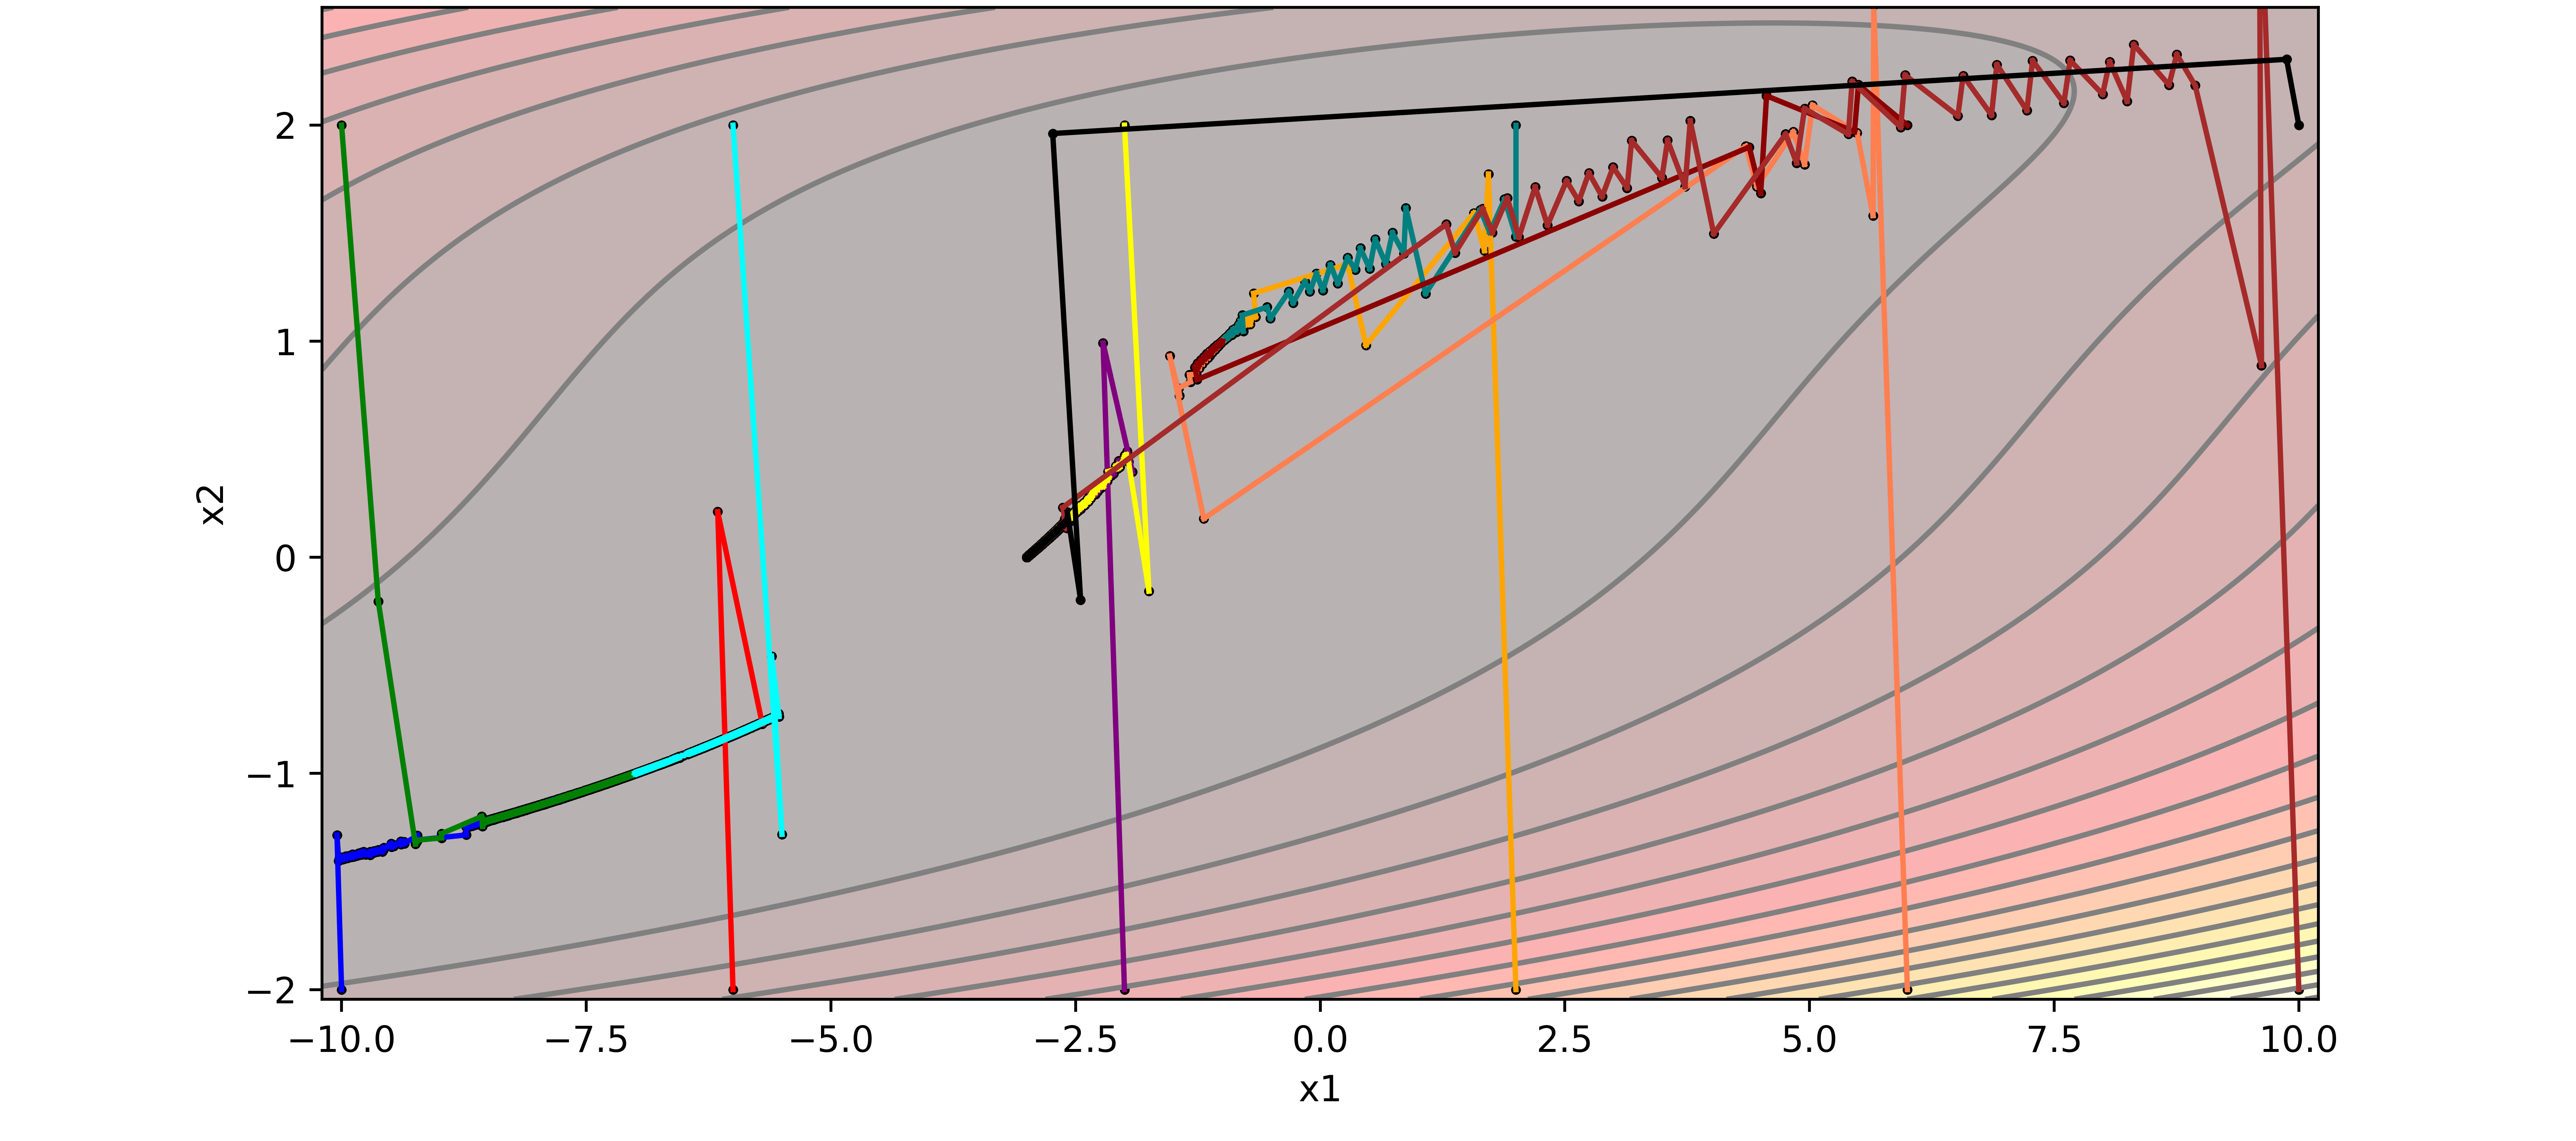
\includegraphics[width=0.9\linewidth]{backtracking}
	\vspace{-5pt}
	\caption{Paths of backtracking with different initial points}
	\label{backtracking}
\end{figure}
\begin{figure}[H]
	\centering
	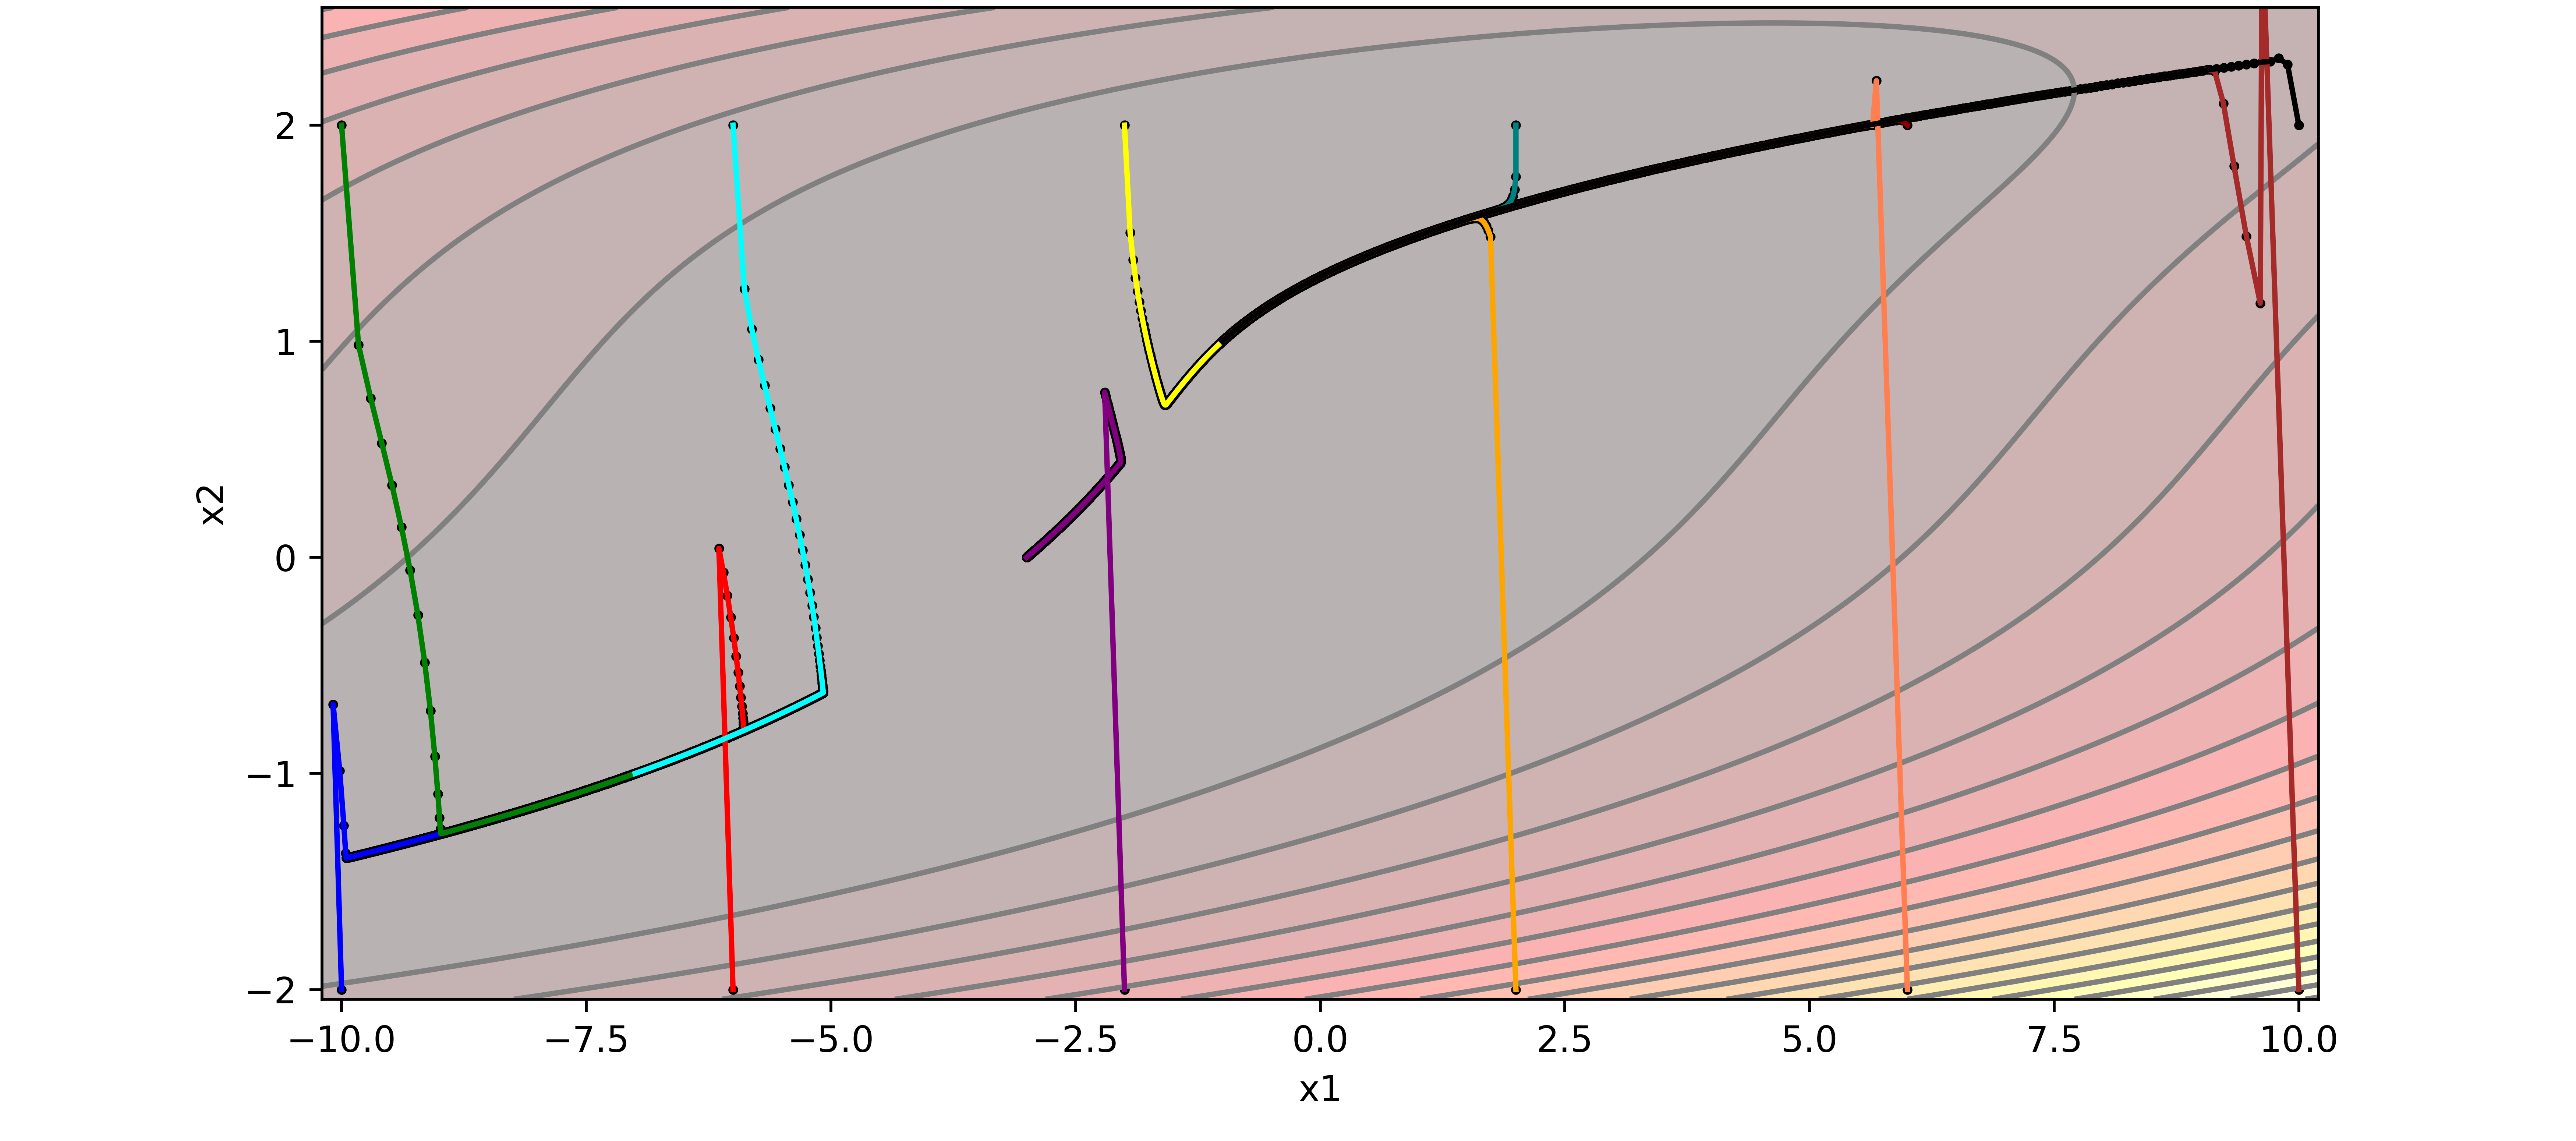
\includegraphics[width=0.9\linewidth]{diminishing}
	\vspace{-5pt}
	\caption{Paths of diminishing step size with different initial points}
	\label{diminishing}
\end{figure}
\begin{figure}[H]
	\centering
	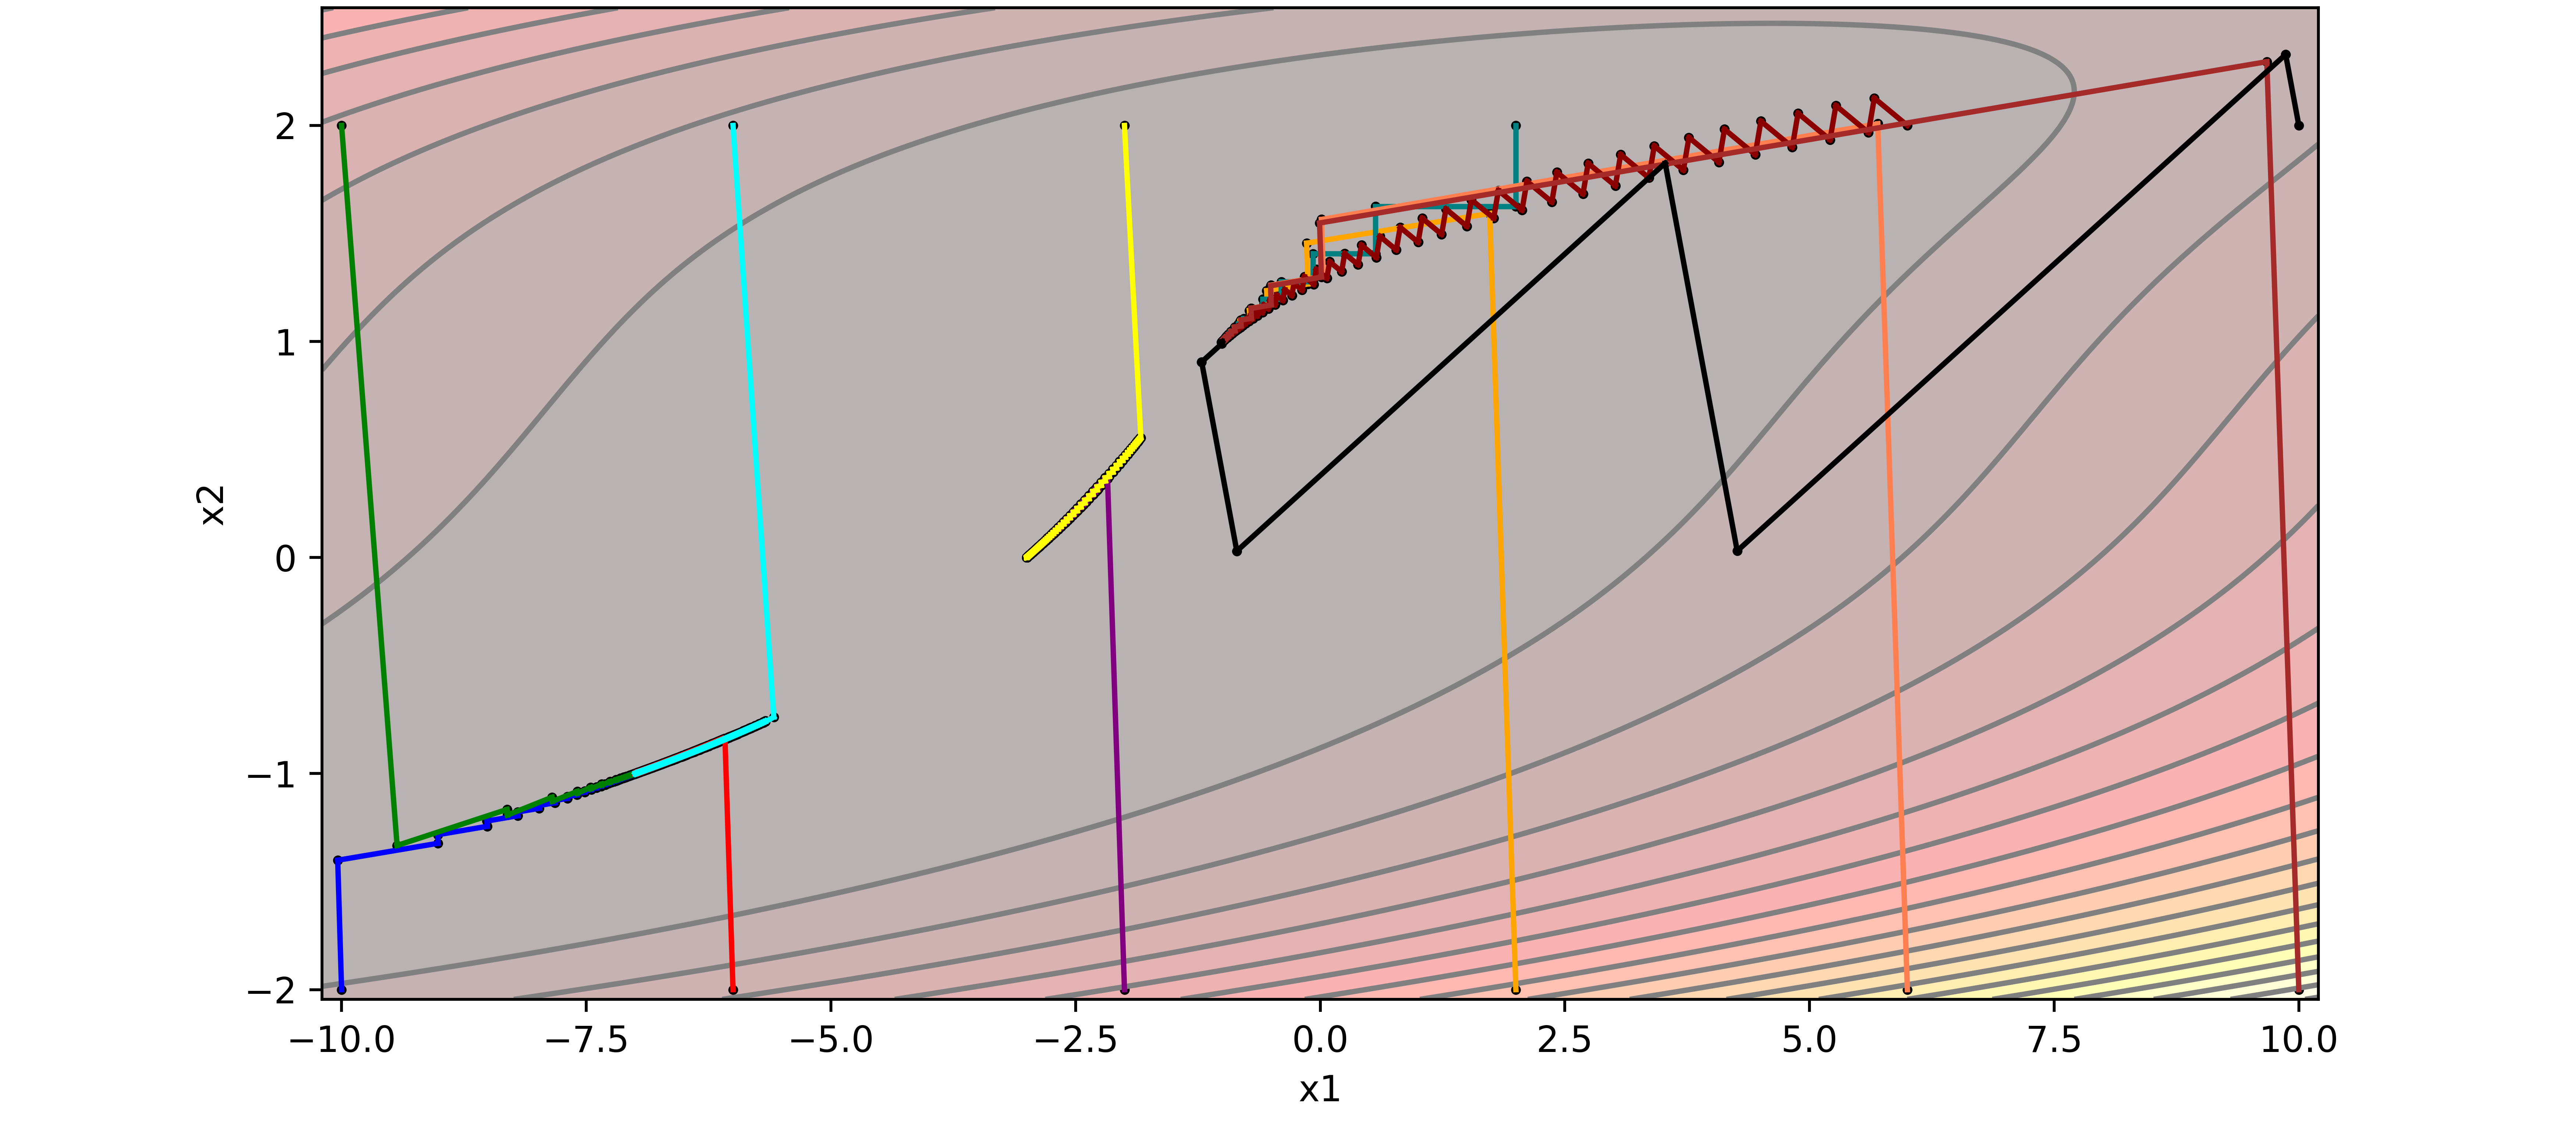
\includegraphics[width=0.9\linewidth]{exact}
	\vspace{-5pt}
	\caption{Paths of exact line search with different initial points}
	\label{exact}
\end{figure}
\begin{python}
# backtracking method
import numpy as np
import matplotlib.pyplot as plt

def f1(x):
    return 3 + x[0] + ((1 - x[1]) * x[1] - 2) * x[1]
def f2(x):
    return 3 + x[0] + (x[1] - 3) * x[1]
def f(x):
    return f1(x) * f1(x) + f2(x) *f2(x)
def df(x):
    grad = np.zeros(2).reshape(2,1)
    grad[0] = 2 * f1(x) + 2 * f2(x)
    grad[1] = 2 * f1(x) * (2*x[1] - 3*(x[1]**2) - 2) + 2 * f2(x) * (2*x[1] - 3)
    return grad
def norm(x):
    return np.sqrt(x[0]**2 + x[1]**2)

color_list = ['blue', 'green', 'red', 'cyan', 'purple', 'yellow', 'orange', 'teal',
              'coral', 'darkred', 'brown', 'black']
def plot_contour():
    X = np.arange(-10.2,10.21,0.05)
    Y = np.arange(-2.045,2.55,0.01125)
    X,Y = np.meshgrid(X,Y)
    Z = np.zeros((X.shape[0], X.shape[1]))
    for i in range(X.shape[0]):
        for j in range(X.shape[1]):
            x = []
            x.append(X[i][j])
            x.append(Y[i][j])
            x = np.array(x)
            Z[i][j] = f(x)
    plt.contourf(X, Y, Z, 20, alpha=0.3, cmap=plt.cm.hot)
    plt.contour(X, Y, Z, 20, colors='grey')
def plot_line(xk_list, subfig_num):
    x = []
    y = []
    for i in range(xk_list.shape[0]):
        x.append(xk_list[i][0][0])
        y.append(xk_list[i][1][0])
    plt.plot(x,y, color = color_list[subfig_num-1], linewidth=1.5)
    plt.scatter(x, y, s=3, color='black')

def gradient_method(initial, subfig_num):
    s = 1
    sigma = 0.5
    gamma = 0.1
    tol = 1e-5
    xk_list = []
    
    xk = initial
    gradient = df(xk)
    num_iteration = 0
    xk_list.append(xk)
    
    while norm(gradient) > tol:
        alphak = s
        dk = -df(xk)
        while True:
            if f(xk + alphak*dk) - f(xk) <= gamma * alphak * np.dot(df(xk).T, dk):
                break
            alphak = alphak * sigma
        xk = xk + alphak * dk
        xk_list.append(xk)
        gradient = df(xk)
        num_iteration = num_iteration + 1
    
    xk_list = np.array(xk_list)
    plot_line(xk_list, subfig_num)
    plt.xlabel('x1')
    plt.ylabel('x2')
    plt.xlim(-10.2, 10.2)
    plt.ylim(-2.045, 2.545)
    
x1 = np.arange(-10, 11, 4)
x2 = np.arange(-2, 3, 4)

plt.figure(1, figsize=(10, 5))
plot_contour()
subfig_num = 1
for i in range(6):
    for j in range(2):
        initial = np.zeros(2).reshape(2,1)
        initial[0] = x1[i]
        initial[1] = x2[j]
        gradient_method(initial, subfig_num)
        subfig_num = subfig_num + 1
plt.savefig('backtracking', dpi=700)       
\end{python}
\begin{python}
# diminishing step size
import numpy as np
import matplotlib.pyplot as plt

def f1(x):
    return 3 + x[0] + ((1 - x[1]) * x[1] - 2) * x[1]
def f2(x):
    return 3 + x[0] + (x[1] - 3) * x[1]
def f(x):
    return f1(x) * f1(x) + f2(x) *f2(x)
def df(x):
    grad = np.zeros(2).reshape(2,1)
    grad[0] = 2 * f1(x) + 2 * f2(x)
    grad[1] = 2 * f1(x) * (2*x[1] - 3*(x[1]**2) - 2) + 2 * f2(x) * (2*x[1] - 3)
    return grad
def norm(x):
    return np.sqrt(x[0]**2 + x[1]**2)
def alpha_k(k):
    return 0.01/(np.log(k+15))

color_list = ['blue', 'green', 'red', 'cyan', 'purple', 'yellow', 'orange', 'teal',
              'coral', 'darkred', 'brown', 'black']
def plot_contour():
    X = np.arange(-10.2,10.21,0.05)
    Y = np.arange(-2.045,2.55,0.01125)
    X,Y = np.meshgrid(X,Y)
    Z = np.zeros((X.shape[0], X.shape[1]))
    for i in range(X.shape[0]):
        for j in range(X.shape[1]):
            x = []
            x.append(X[i][j])
            x.append(Y[i][j])
            x = np.array(x)
            Z[i][j] = f(x)
    plt.contourf(X, Y, Z, 20, alpha=0.3, cmap=plt.cm.hot)
    plt.contour(X, Y, Z, 20, colors='grey')
def plot_line(xk_list, subfig_num):
    x = []
    y = []
    for i in range(xk_list.shape[0]):
        x.append(xk_list[i][0][0])
        y.append(xk_list[i][1][0])
    plt.plot(x,y, color = color_list[subfig_num-1], linewidth=1.5)
    plt.scatter(x, y, s=3, color='black')

def gradient_method(initial, subfig_num):
    tol = 1e-5
    num_iteration = 0
    k = 1
    xk = initial
    gradient = df(xk)
    xk_list = []
    xk_list.append(xk)
  
    while norm(gradient) > tol:
        dk = -df(xk)
        alphak = alpha_k(k)
        xk = xk + alphak * dk
        xk_list.append(xk)
        gradient = df(xk)
        num_iteration = num_iteration + 1
        k = k + 1
        
    xk_list = np.array(xk_list)
    plot_line(xk_list, subfig_num)
    plt.xlabel('x1')
    plt.ylabel('x2')
    plt.xlim(-10.2, 10.2)
    plt.ylim(-2.045, 2.545)
    
x1 = np.arange(-10, 11, 4)
x2 = np.arange(-2, 3, 4)

plt.figure(1, figsize=(10, 5))
plot_contour()
subfig_num = 1

for i in range(6):
    for j in range(2):
        initial = np.zeros(2).reshape(2,1)
        initial[0] = x1[i]
        initial[1] = x2[j]
        gradient_method(initial, subfig_num)
        subfig_num = subfig_num + 1
plt.savefig('diminishing', dpi=700)                 
\end{python}
\begin{python}
# exact line search
import numpy as np
import matplotlib.pyplot as plt

def f1(x):
    return 3 + x[0] + ((1 - x[1]) * x[1] - 2) * x[1]
def f2(x):
    return 3 + x[0] + (x[1] - 3) * x[1]
def f(x):
    return f1(x) * f1(x) + f2(x) *f2(x)
def df(x):
    grad = np.zeros(2).reshape(2,1)
    grad[0] = 2 * f1(x) + 2 * f2(x)
    grad[1] = 2 * f1(x) * (2*x[1] - 3*(x[1]**2) - 2) + 2 * f2(x) * (2*x[1] - 3)
    return grad
def norm(x):
    return np.sqrt(x[0]**2 + x[1]**2)

color_list = ['blue', 'green', 'red', 'cyan', 'purple', 'yellow', 'orange', 'teal',
              'coral', 'darkred', 'brown', 'black']
def plot_contour():
    X = np.arange(-10.2,10.21,0.05)
    Y = np.arange(-2.045,2.55,0.01125)
    X,Y = np.meshgrid(X,Y)
    Z = np.zeros((X.shape[0], X.shape[1]))
    for i in range(X.shape[0]):
        for j in range(X.shape[1]):
            x = []
            x.append(X[i][j])
            x.append(Y[i][j])
            x = np.array(x)
            Z[i][j] = f(x)
    plt.contourf(X, Y, Z, 20, alpha=0.3, cmap=plt.cm.hot)
    plt.contour(X, Y, Z, 20, colors='grey')
def plot_line(xk_list, subfig_num):
    x = []
    y = []
    for i in range(xk_list.shape[0]):
        x.append(xk_list[i][0][0])
        y.append(xk_list[i][1][0])
    plt.plot(x,y, color = color_list[subfig_num-1], linewidth=1.5)
    plt.scatter(x, y, s=3, color='black')

def gradient_method(initial, subfig_num):
    tol = 1e-5
    xk = initial
    gradient = df(xk)
    num_iteration = 0
    tol_golden = 1e-6
    maxit = 100
    a = 2
    xk_list = []
    xk_list.append(xk)
        
    while norm(gradient) > tol:
        dk = -df(xk)
        alphal = 0
        alphar = a
        num_iteration_golden = 0
        last_update = 0 #0:left; 1:right
        fi = (3 - np.sqrt(5)) / 2
        while (alphar - alphal) >= tol_golden and num_iteration_golden < maxit:
            if num_iteration_golden == 0:
                new_alphal = fi * alphar + (1 - fi) * alphal
                new_alphar = (1 - fi) * alphar + fi * alphal
            elif last_update == 0:
                new_alphal = new_alphar
                new_alphar = (1 - fi) * alphar + fi * alphal
            else:
                new_alphar = new_alphal
                new_alphal = fi * alphar + (1 - fi) * alphal
            
            f_alphal = f(xk + new_alphal*dk)
            f_alphar = f(xk + new_alphar*dk)
            
            if f_alphal < f_alphar:
                alphar = new_alphar
                last_update = 1
            else:
                alphal = new_alphal
                last_update = 0
            num_iteration_golden = num_iteration_golden + 1
        alphak = (alphal + alphar) / 2
        xk = xk + alphak * dk
        xk_list.append(xk)
        gradient = df(xk)
        num_iteration = num_iteration + 1
    
    xk_list = np.array(xk_list)
    plot_line(xk_list, subfig_num)
    plt.xlabel('x1')
    plt.ylabel('x2')
    plt.xlim(-10.2, 10.2)
    plt.ylim(-2.045, 2.545)
    
x1 = np.arange(-10, 11, 4)
x2 = np.arange(-2, 3, 4)

plt.figure(1, figsize=(10, 5))
plot_contour()
subfig_num = 1
for i in range(6):
    for j in range(2):
        initial = np.zeros(2).reshape(2,1)
        initial[0] = x1[i]
        initial[1] = x2[j]
        gradient_method(initial, subfig_num)
        subfig_num = subfig_num + 1
plt.savefig('exact', dpi=700)        
\end{python}
\end{homeworkProblem}
\end{document}

